\RequirePackage[dvipsnames,hyperref,table]{xcolor}
\documentclass[a4paper,11pt,twoside]{scrartcl}
%
%      Copyright (C) Ferréol Soulez, 2020 
%      ferreol.soulez@univ-lyon1.fr
%
%     This program is free software: you can redistribute it and/or modify
%     it under the terms of the GNU General Public License as published by
%     the Free Software Foundation, either version 3 of the License, or
%     (at your option) any later version.
%
%     This program is distributed in the hope that it will be useful,
%     but WITHOUT ANY WARRANTY; without even the implied warranty of
%     MERCHANTABILITY or FITNESS FOR A PARTICULAR PURPOSE.  See the
%     GNU General Public License for more details.
%
%     You should have received a copy of the GNU General Public License
%     along with this program.  If not, see <http://www.gnu.org/licenses/>.
%
%% Ferréol Soulez, 2020

\usepackage{amsmath,amsfonts,amssymb,textcomp,mathtools}
\usepackage{mathrsfs}
\usepackage{xspace} 


\makeatletter \newcommand{\MathFuncName}[1]{{\operator@font #1}}
\newcommand{\MathFunc}[1]{\mathop{\operator@font #1}\nolimits}
\newcommand{\MathFuncWithLimits}[1]{\mathop{\operator@font #1}\limits}
\makeatother

\newcommand{\asterisk}{*}
\newcommand{\mathd}{\mathrm{d}} % roman 'd' for integrand/differential
\newcommand{\mathe}{\mathrm{e}} % roman 'e' for exp(1)
\newcommand{\mathi}{\mathrm{i}} % roman 'i' for sqrt(-1)

\newcommand{\BF}[1]{\mathbf{#1}} % math bold
\newcommand{\RM}[1]{\mathrm{#1}} % math roman
\newcommand{\SF}[1]{\mathsf{#1}} % math sans-serif
\newcommand{\OP}[1]{{\MathFuncName{#1}}} % upright (*) for function names
\newcommand{\Tag}[1]{\mathsf{#1}} % math font for labels and tags
\newcommand{\BS}[1]{{\boldsymbol{#1}}} % bold symbol (*)
\newcommand{\V}[1]{\boldsymbol{#1}} % vector
\newcommand{\M}[1]{\mathbf{#1}} % matrix
\newcommand{\Inner}[2]{\left \langle #1,#2 \right\rangle} % Inner product
% \newcommand{\TransposeLetter}{\mathrm{T}}
% \newcommand{\TransposeLetter}{\mathsf{t}}
% \newcommand{\TransposeLetter}{{\intercal}}
% \newcommand{\TransposeLetter}{\top}
\newcommand{\AdjointLetter}{\dagger}
\newcommand{\T}{^{\AdjointLetter}} % suffix for transpose
\newcommand{\TransposeLetter}{\top}
\newcommand{\Tt}{^{\TransposeLetter}} % suffix for transpose
\newcommand{\mT}{^{-\TransposeLetter}} % suffix for inverse transpose
\newcommand{\I}{\mathi} % roman 'i' for sqrt(-1)
\newcommand{\E}{\mathe} % roman 'e' for exp(1)
\newcommand{\D}[1]{{\mathd #1}} % integrand/differential
\newcommand{\ScaleAs}{\mathcal{O}} % O(n)
\renewcommand{\Re}{\MathFunc{Re}} % real part
\newcommand{\sign}{\MathFunc{sign}} % sign
\newcommand{\Arg}{\MathFunc{Arg}} % argument
%\newcommand{\mod}{\MathFunc{mod}} % modulo
\renewcommand{\Im}{\MathFunc{Im}} % imaginary part
\newcommand{\arc}{\MathFunc{arc}} % lenght of arc
\newcommand{\rect}{\MathFunc{rect}} % real part
\newcommand{\rnd}{\MathFunc{rnd}} % random
\newcommand{\sgn}{\MathFunc{sgn}} % sign function
\newcommand{\sinc}{\MathFunc{sinc}} % cardinal sine
\newcommand{\asin}{\MathFunc{asin}} % inverse sine
\newcommand{\acos}{\MathFunc{acos}} % inverse cosine
\newcommand{\Var}{\MathFunc{Var}} % variance
\newcommand{\Cov}{\MathFunc{Cov}} % covariance
\DeclarePairedDelimiterXPP{\Expect}[1]{\mathrm{E}}(){}{#1}
\newcommand*{\delimsize}{}
\newcommand*{\given}{\,\vert\,} % compact version
\newcommand*{\Given}{\:\delimsize\vert\:} % autoscale to surrounding version

\newcommand{\Card}{\MathFunc{Card}} % cardinal, number of elements
\newcommand{\diag}{\MathFunc{diag}} % diagonal
\newcommand{\eig}{\MathFunc{eig}} % eigenvalues
\newcommand{\tr}{\MathFunc{tr}} % trace
\newcommand{\rank}{\MathFunc{rank}} % rank
\newcommand{\pdf}{\MathFunc{pdf}} % probability density function
\newcommand{\para}{{/\!/}} % parallel
\newcommand{\prox}{\operatorname{prox}} % proximity operator
\newcommand{\conj}[1]{\operatorname{conj}\Paren{#1}} % proximity operator
\newcommand{\proxy}[1]{\widetilde{#1}} % approximation
% (*) enclosed in braces so that x_\BS{u} or x_\RM{name} works
\newcommand{\comp}{\mathop{\circ}}



% Partial derivative:
\newcommand{\PDer}[2]{\frac{\partial #1}{\partial #2}}
\newcommand{\At}[2]{\left.#1\right\vert_{#2}}

\newcommand{\Paren}[1]{\left(#1\right)}
\newcommand{\bigParen}[1]{\bigl(#1\bigr)}
\newcommand{\BigParen}[1]{\Bigl(#1\Bigr)}

\newcommand{\Brace}[1]{\left\{#1\right\}}
\newcommand{\bigBrace}[1]{\bigl\{#1\bigr\}}
\newcommand{\BigBrace}[1]{\Bigl\{#1\Bigr\}}

\newcommand{\SqBrack}[1]{\left[#1\right]}
\newcommand{\bigSqBrack}[1]{\bigl[#1\bigr]}
\newcommand{\BigSqBrack}[1]{\Bigl[#1\Bigr]}

% Norm, e.g. ||x|| (fixed and scalable):
\newcommand{\norm}[1]{\Vert #1\Vert} 
\newcommand{\Norm}[1]{\left\Vert #1\right\Vert}
\newcommand{\bigNorm}[1]{\bigl\Vert #1\bigr\Vert}
\newcommand{\BigNorm}[1]{\Bigl\Vert #1\Bigr\Vert}

% Absolute value, e.g. |x| (fixed and scalable):
\newcommand{\abs}[1]{\vert #1\vert} 
\newcommand{\Abs}[1]{\left\vert #1\right\vert} \newcommand{\bigAbs}[1]{\bigl\vert #1\bigr\vert}
\newcommand{\BigAbs}[1]{\Bigl\vert #1\Bigr\vert}

% Average value, e.g. <x> (fixed and scalable):
\newcommand{\avg}[1]{\langle #1\rangle}
\newcommand{\Avg}[1]{\left\langle #1\right\rangle}
\newcommand{\bigAvg}[1]{\bigl\langle #1\bigr\rangle}
\newcommand{\BigAvg}[1]{\Bigl\langle #1\Bigr\rangle}

% Complex quantity:
\newcommand{\complex}[1]{\underline{#1}}

% For optimization problems, "arg min" and "arg max":
\newcommand{\argmin}{\MathFuncWithLimits{arg\,min}}
\newcommand{\argmax}{\MathFuncWithLimits{arg\,max}}
\newcommand{\minimize}{\MathFuncWithLimits{minimize}}
\newcommand{\find}{\MathFuncWithLimits{find}}

% Marker for end of proof/algorithm:
\newcommand{\EndProof}{\ensuremath{\blacksquare}}
% \newcommand{\EndProof}{\ensuremath{Box{}}} Quadratic term:
\newcommand{\QuadTerm}[2]{#2\T\!\!\cdot #1\cdot #2}

% Fourier transforms:
\newcommand{\FT}[1]{\widehat{#1}} % Fourier transform
\newcommand{\TwoIPi}{2\,\I\,\pi} % 2*i*pi
\newcommand{\F}[1]{\mathcal{F}\Paren{#1}}
\newcommand{\IF}[1]{\mathcal{F}^{-1}\Paren{#1}}
\newcommand{\FTarrow}{\xrightarrow{\mathrm{FT}}}
\newcommand{\DFTarrow}{\xrightarrow{\mathrm{DFT}}}

% Sets:
\newcommand{\Set}[1]{\mathbb{#1}} \newcommand{\Reals}{\mathbb{R}}
\newcommand{\Integers}{\mathbb{Z}} \newcommand{\Natural}{\mathbb{N}}
\newcommand{\Complexes}{\mathbb{C}}
\newcommand{\Rationals}{\mathbb{Q}}

% By definition: \newcommand\bydef{\equiv}
% \newcommand\bydef{\triangleq}
\newcommand{\bydef}{\stackrel{\text{\tiny def}}{=}}

\newcommand\BesselJ[1]{\mathop{\mathrm{J}}\nolimits_{#1}}


\renewcommand{\Re}{\MathFunc{Re}}        % real part
\renewcommand{\Im}{\MathFunc{Im}}        % imaginary part


\newcommand{\Eq}[1]{Eq.~(\ref{#1})}
\newcommand{\Fig}[1]{Fig.~\ref{#1}}


% Common abbreviation:
\newcommand{\cf}{\emph{cf.}\xspace}
\newcommand{\eg}{\emph{e.g.}\xspace}
\newcommand{\ie}{\emph{i.e.}\xspace} \newcommand{\etal}{\emph{et
    al.}\xspace} \newcommand{\etc}{\emph{etc.}\xspace}
\newcommand{\wrt}{with respect to\xspace}


\usepackage[utf8]{inputenc}
\usepackage[T1]{fontenc}
\usepackage{stmaryrd}


\renewcommand{\AdjointLetter}{\mathrm{T}}
\usepackage{lmodern}
\DeclareUnicodeCharacter{00B5}{\ensuremath{\mu}} % µ
\DeclareUnicodeCharacter{2264}{\ensuremath{\le}} % ≤
\DeclareUnicodeCharacter{2265}{\ensuremath{\ge}} % ≥
\DeclareUnicodeCharacter{22C5}{\!\cdot\!}
\usepackage{graphicx} % Required for inserting images


\title{Notes about GRAVITY+ metrology demodulation}


\author{Ferréol Soulez }
\date{February 2023}

\begin{document}

\maketitle

\section{The metrology table}
The metrology data is stored as a FITS Table in the \verb+METROLOGY+ HDU (10$^\textrm{th}$) as in table \ref{tab:table}. The voltages \verb+VOLT+ are composed of $80$ columns:
\begin{itemize}
    \item 2 directions ($x$ and  $y$) per diodes
    \item 4 diodes per telescope (one on each spiders)
    \item 1 fiber coupler diode (labeled \verb+FC+) per telescope
    \item 4 telescopes
    \item 2 sides: \verb|FT|  and \verb|SC|
\end{itemize}
The signals (the table column) are sample at $500\,$Hz leading to a very large number of rows. 
\begin{table}[]
    \centering
    \begin{tabular}{l| l ll}
Name   &       Size  & Type  &   TFORM   \\
\hline
TIME   &              & Int32  &  1J     \\
VOLT   &       (80,) & Float32 &  80E    \\
POWER\_LASER   &    &   Float32 & 1E     \\
LAMBDA\_LASER   &    &  Float32 & 1E     
    \end{tabular}
    \caption{Metrology table}
    \label{tab:table}
\end{table}

\section{The modulation model}

When the pupil modulation is on (\verb|ESO INS PMC1 MODULATE| keyword is \verb|true|), the metrology signal is modulated at a frequency of $f=1\,$Hz. 
This modulation does not affect the fiber coupler diode.

For each diode in \{D1, D2, D3, D4\}, we define the complex measurement $\V{v} \in \Complexes^N$  with $v_i =   x_i + \jmath y_i \,, \quad \forall i \in \llbracket 1,N \rrbracket $ and  $N$ is the number of row of the metrology. The modulation as a function of time is:
\begin{equation}
    \V{v} = \exp\left( \jmath \, b \sin\left( \V{\omega} + \phi\right)\right)\,.\label{eq:v}
\end{equation}
where $\omega = 2\,\pi\,\V{t}$ is the modulation pulsation built from the \verb|TIME| column, the amplitude $b$  and the phase $\phi$  are the modulation parameters to be estimated to demodulate the metrology signal.


\section{The overall model}
For a  diode the measured modulated voltage data $\V{d}$ can be modeled by:
\begin{equation}
    \V{d} = \left( c + \V{s} \times  \exp\left( \jmath \, b \sin\large( \V{\omega} + \phi\large)\right)\right)\times\exp\left(\jmath\,\Phi_\textrm{FC}\right)+  \V{e}\,,\label{eq:model}
\end{equation}
where $\times$ is the element-wise multiplication, $\V{s}$ is the sought-after demodulated  metrology signal, $\Phi_\textrm{FC}$ is the phase of the fiber coupler measurement accounting for FDDL movements. $c  = x_0 + \jmath\,y_0$ is the center of the pupil and $\V{e}$ is a vector representing the errors on the measurement that are supposed Gaussian centered, independent and identically distributed.



\section{ Estimating the modulation parameters}

To estimate the modulation parameters we need to disentangle it from the signal  $\V{s}$. This is done using the expansion:
\begin{equation}
    \V{s} = a  + \V{\delta v}\,
\end{equation}
$\abs{a}$  and $\arg{(a)}$ being the  mean amplitude and phase respectively of the metrology signal.  $ \V{\delta v}$ is centered ($\Expect{\delta v}= 0$)  and supposed to be Gaussian independant and identically distributed.

Under this assumption, the modulation parameters $( b, \phi)$, the center $c$ and the mean of the metrology signal $a$ can be estimated using least square:
\begin{equation}
    (c^+, a^+, b^+, \phi^+) = \argmin_{c,a,b,\phi} \Norm{\V{d} -  \left(c + a \exp\left( \jmath \, b \sin\Large( \V{\omega} + \phi\right)\Large)\right)\times\exp\left(\jmath\,\Phi_\textrm{FC}\right) }_2^2
\end{equation}
that is equivalent with : 
\begin{equation}
    (c^+, a^+, b^+, \phi^+) = \argmin_{c,a,b,\phi} \Norm{\V{r} -  c - a \exp\left( \jmath \, b \sin\left( \V{\omega} + \phi\right)\right) }_2^2\label{eq:r}
\end{equation}
with $\V{r} =\V{d}\times\exp\left(-\jmath\,\Phi_\textrm{FC}\right)$.

\subsection{Linear estimates}
From the equation \ref{eq:r}, we can see that the parameters  $c$ and $a$ depends linearly of the  $\V{d}$ and the modulation phasor $\V{m} = \exp\left( \jmath \, b \sin\left( \V{\omega} + \phi\right)\right)$. For a given values of $b$ and $\phi$, the optimal values $c^+$ and $a^+$ have a closed-form solution that is:
\begin{equation}
    \left[\begin{array}{l}
    c^+\\
    a^+
    \end{array}\right] = \M{A}^{-1} 
    \left[\begin{array}{l}
    \sum_i d_i\\
    \V{m}\T\V{d}
    \end{array}\right] 
\end{equation}
where $\V{m}\T$ is the conjugate transpose of $\V{m}$ and $\M{A}$ is the $2\times2$ matrix:
\begin{equation}
    \M{A} = \left[\begin{array}{ll}
    N & \sum_i m_i\\
    \sum_i  m_i^* & N
    \end{array}\right] \,,
\end{equation}
where $m_i^*$ is the complex conjugate of $m_i$ and $N$  the number of measurements. Its inverse is:
\begin{equation}
   \M{A}^{-1} \frac{1}{N^2 \left(1 - \Abs{ \sum_i d_i}^2\right)}\,\left[\begin{array}{ll}
    N & - \sum_i m_i\\
    - \sum_i  m_i^* & N
    \end{array}\right] 
\end{equation}
For a couple $(b,\phi)$ the optimal $c^+(b,\phi)$ and $a^+(b,\phi)$ is given by:
\begin{align}
    c^+(b,\phi) &= \frac{N\,\sum_i d_i - \V{m}\T\V{d}\sum_i m_i}{N^2 \left(1 - \Abs{ \sum_i d_i}^2\right)}\\
    a^+(b,\phi) &= \frac{ -N\,\left(\sum_i d_i\right)  \left(\sum_i  m_i^*\right)+ \V{m}\T\V{d}}{N^2 \left(1 - \Abs{ \sum_i d_i}^2\right)}
\end{align}

\subsection{Non-linear estimates}
The modulation parameters estimation amounts to estimate only $b$  and $\phi$, optimizing the function:
\begin{equation}
   f(b,\phi) = \Norm{\V{r} -  c^+(b,\phi) - a^+(b,\phi) \exp\left( \jmath \, b \sin\left( \V{\omega} + \phi\right)\right) }_2^2\label{eq:nl}
\end{equation}
\begin{figure}
    \centering
    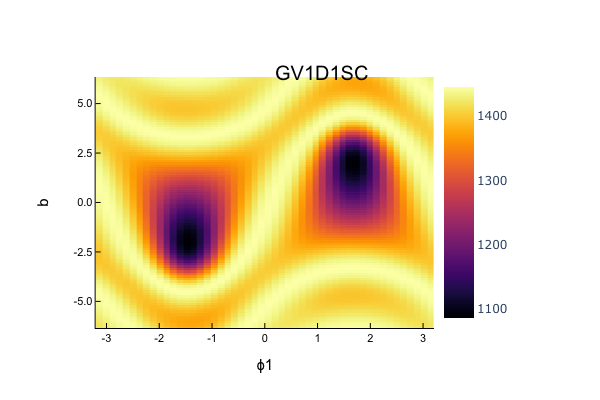
\includegraphics[width=0.45\linewidth]{figs/GV1D1SC.png}
    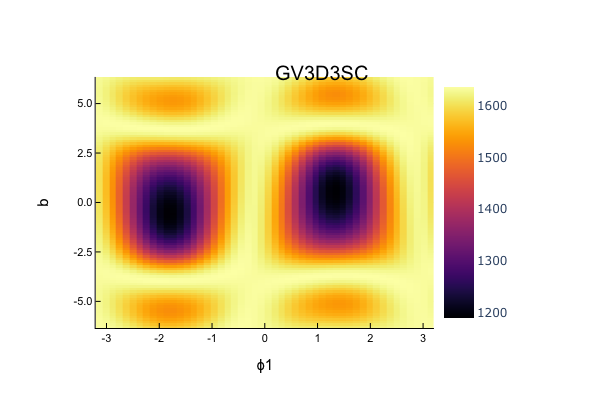
\includegraphics[width=0.45\linewidth]{figs/GV3D3SC.png}
    \caption{$f(b,\phi)$ for two different diodes}
    \label{fig:GV1D1SC}
\end{figure}

This function is non-linear and non-convex as it can be seen on figure \ref{fig:GV1D1SC}. The two main optimum are equivalent as $f(b,\phi) f(-b,\phi+ \pi )$ An initialization with $b$ sufficiently small seems to ensure to end in the global optimum. Note that the case $b=0$ is singular  as $f(b,\phi)$ is equal to the variance of $\V{r}$ in this case whatever is $\phi$, $a$ and $ c$.

In the code this function is minimizes by the mean of the derivative free NEWOA method of powel that seems faster than VMLMB (with derivative) and  the Simplex method.
\section{Demodulation}
Once the modulation parameters are estimated the demodulated signal is given by:
\begin{equation}
\V{s} =\left(\V{r} - c^+\right)\times\exp\left( \jmath \, b^+ \sin\large( \V{\omega} + \phi^+_1\large)\right)\times\exp\left(\jmath\,\Phi_\textrm{FC}\right)\,,\label{eq:demodulation}
\end{equation}

All the $6\times4\times4\times2$ parameters are stored in keywords of the METROLOGY table header as shown on the table \ref{tab:keyword}. These keywords are suffixed with the side, the telescope number and the diode (\eg \verb|DEMODULATION CENTER X0 SC T4 D1|).
\begin{table}[]
    \centering
    \begin{tabular}{l c l}
Name   &          & keyword   \\
center    &      $\Re(c^+)$        &   \verb|DEMODULATION CENTER X0|   \\
center   &      $\Im(c^+) $       &   \verb|DEMODULATION CENTER Y0|   \\
metrology amplitude  &      $\Abs{a^+} $       &   \verb|DEMODULATION AMPLITUDE ABS|   \\
metrology phase  &      $\arg{(a^+)} $       &   \verb|DEMODULATION AMPLITUDE ARG|   \\
modulation amplitude  &      $b^+ $       &   \verb|DEMODULATION SIN AMPLITUDE |   \\
modulation phase  &      $\phi^+ $       &   \verb|DEMODULATION SIN PHASE|   
    \end{tabular}
    \caption{Metrology table}
    \label{tab:keyword}
\end{table}
\end{document}
